\section{アプローチ04（骨格検出（ポーズ推定）に基づく人物検出手法）}

\subsection{手法の概要}
アプローチ03で判明した「後ろ姿や横顔における顔検出の漏れ」および「身体の向き・姿勢情報の不足」に対応するため、アプローチ04では人物の検出基準を「顔」から「骨格（ポーズ領域）」へ移行した。

ポーズ推定モデルを用いて身体の関節点（キーポイント）を抽出し、頭部・肩・胴体等の骨格情報の配置パターンから人物の存在判定および領域推定を行う。これにより、顔が遮蔽されている場合やカメラに対して後方・側方を向いている人物であっても、一貫した検出が可能となる。

\subsection{実験結果およびアプローチ03との比較・課題}

\subsubsection{実験結果}
静止画を入力データとして検証を行った際の実験結果を表\ref{tab:approach04_image_results}に示す。
なお、いずれの実験結果においても、緑色のバウンディングボックスは検出された人物、赤色のバウンディングボックスは同定されたグループを示している。

\begin{table}[H]
  \centering
  \small
  \caption{アプローチ04：実験結果の比較（静止画）}
  \label{tab:approach04_image_results}
  \adjustbox{max width=\textwidth}{%
  \begin{tabular}{|c|c|c|c|c|}
    
    \hline

      & \begin{tabular}{c} 前アプローチの \\ 検出結果 \end{tabular}
      & 検出結果
      & \begin{tabular}{c} 検出された \\ グループ数 \end{tabular}
      & 実際のグループ数との差 \\
    
    \hline
    
    $\vcenter{\hbox{標準状態}}$ &
      $\vcenter{\hbox{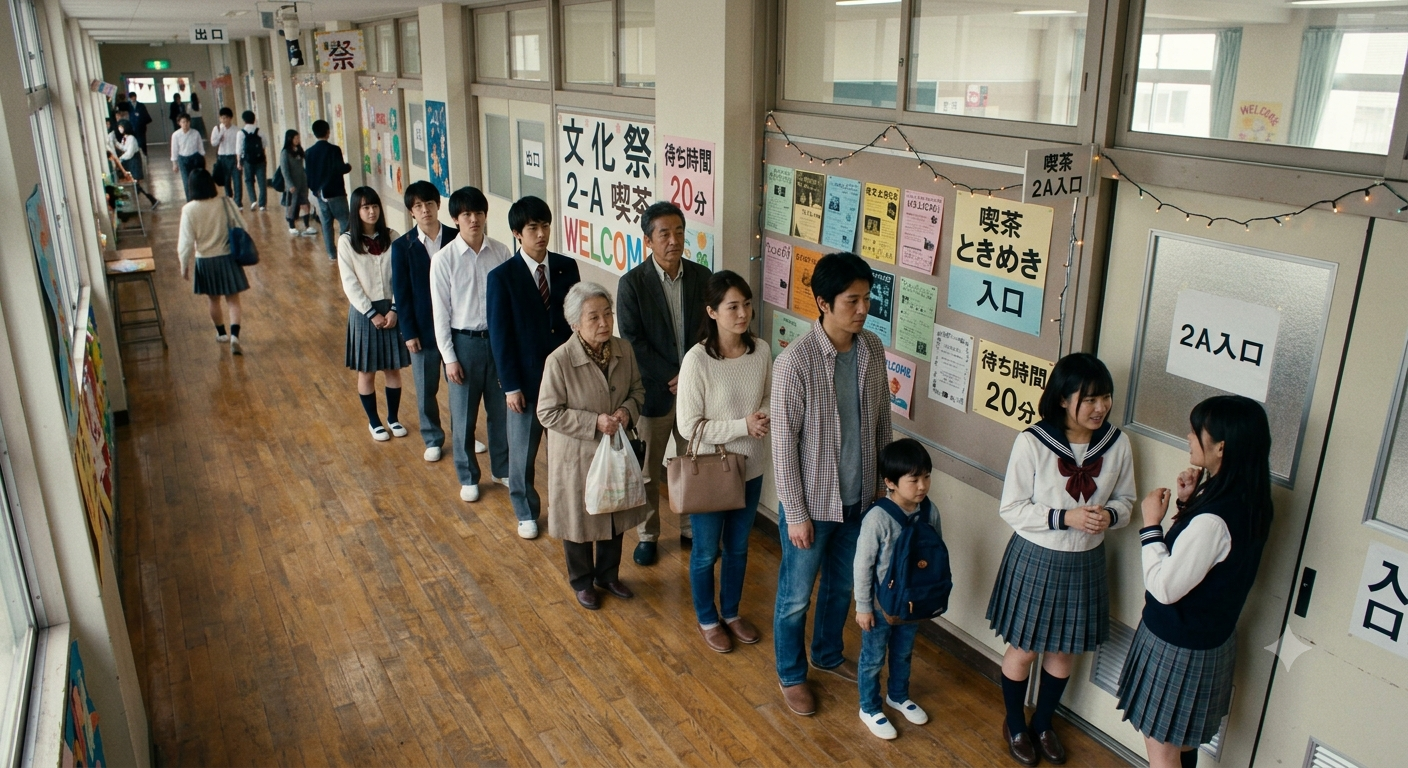
\includegraphics[width=0.25\textwidth]{experiment/results/approach_03_face_detection/standard/detection_outputs/annotated_images/t_001s.png}}}$ &
      $\vcenter{\hbox{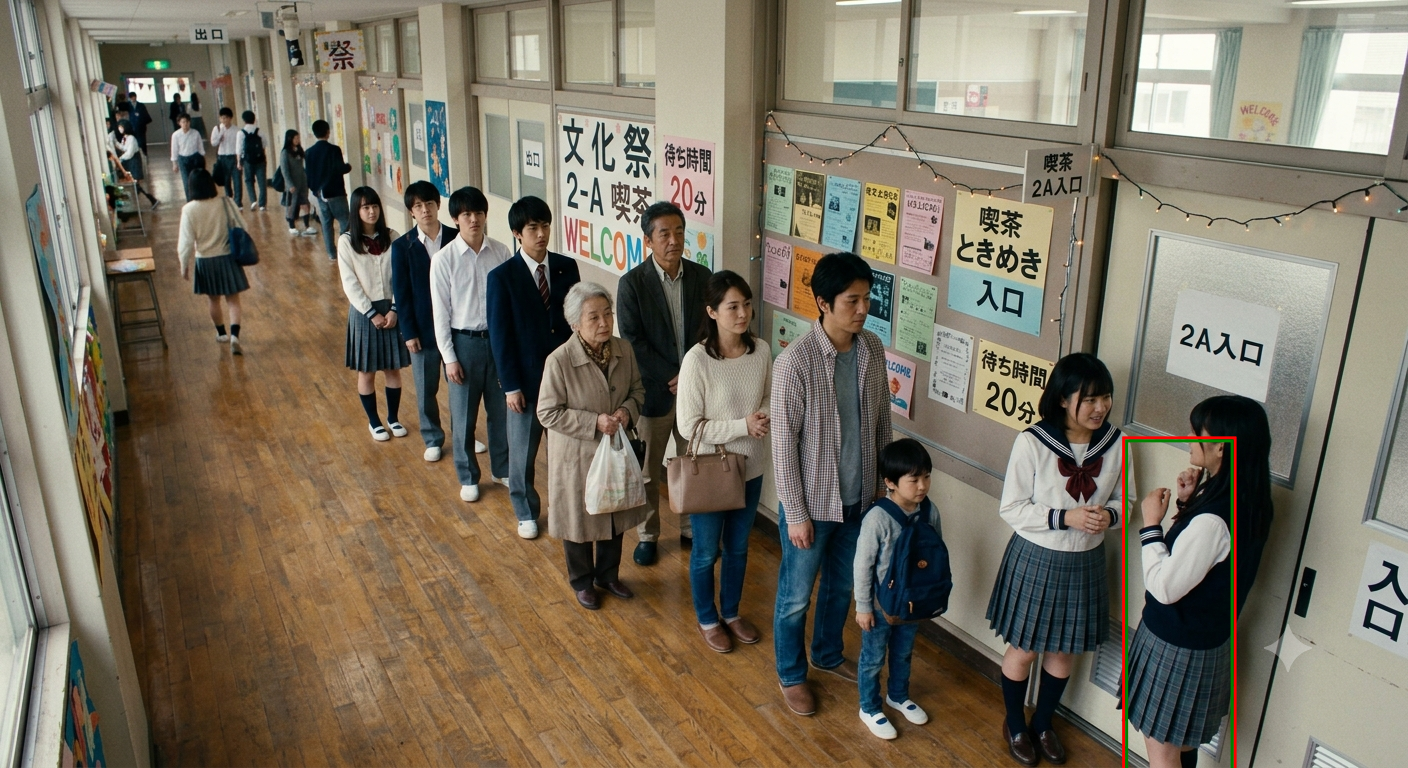
\includegraphics[width=0.25\textwidth]{experiment/results/approach_04_pose_detection/standard/detection_outputs/annotated_images/t_001s.png}}}$ &
      \jsonlen{experiment/results/approach_04_pose_detection/standard/detection_outputs/labels/t_001s.json} &
      % 符号と数値
        \ifnum\numexpr \jsonlen{experiment/results/approach_04_pose_detection/standard/detection_outputs/labels/t_001s.json} - \gtstandard\relax>0 +\fi\the\numexpr
        \jsonlen{experiment/results/approach_04_pose_detection/standard/detection_outputs/labels/t_001s.json} - \gtstandard\relax \\
    
    \hline
    
    $\vcenter{\hbox{密集状態}}$ &
      $\vcenter{\hbox{\includegraphics[width=0.25\textwidth]{experiment/results/approach_03_face_detection/crowded/detection_outputs/annotated_images/t_001s.png}}}$ &
      $\vcenter{\hbox{\includegraphics[width=0.25\textwidth]{experiment/results/approach_04_pose_detection/crowded/detection_outputs/annotated_images/t_001s.png}}}$ &
      \jsonlen{experiment/results/approach_04_pose_detection/crowded/detection_outputs/labels/t_001s.json} &
      % 符号と数値
        \ifnum\numexpr \jsonlen{experiment/results/approach_04_pose_detection/crowded/detection_outputs/labels/t_001s.json} - \gtcrowded\relax>0 +\fi\the\numexpr
        \jsonlen{experiment/results/approach_04_pose_detection/crowded/detection_outputs/labels/t_001s.json} - \gtcrowded\relax \\
    
    \hline
    
    $\vcenter{\hbox{非組織群集}}$ &
      $\vcenter{\hbox{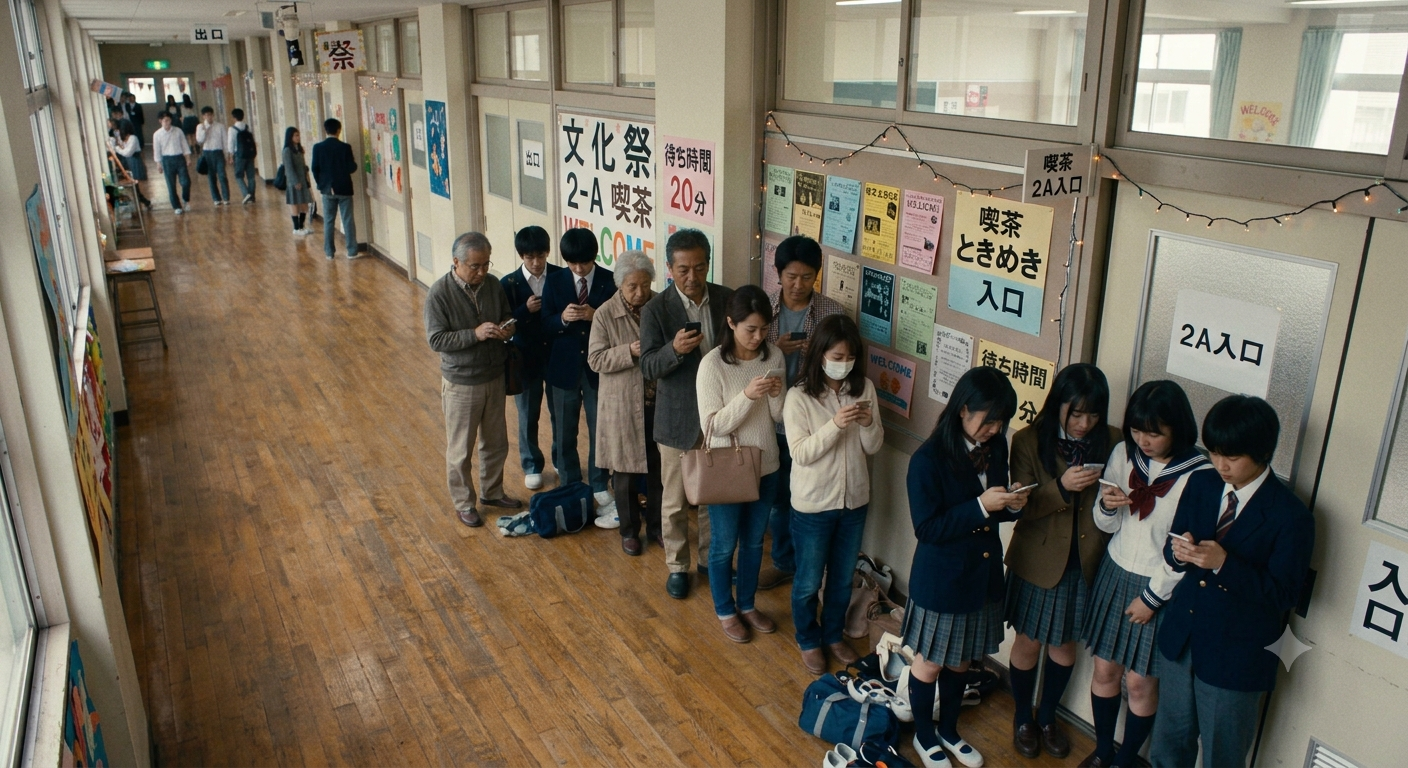
\includegraphics[width=0.25\textwidth]{experiment/results/approach_03_face_detection/strangers/detection_outputs/annotated_images/t_001s.png}}}$ &
      $\vcenter{\hbox{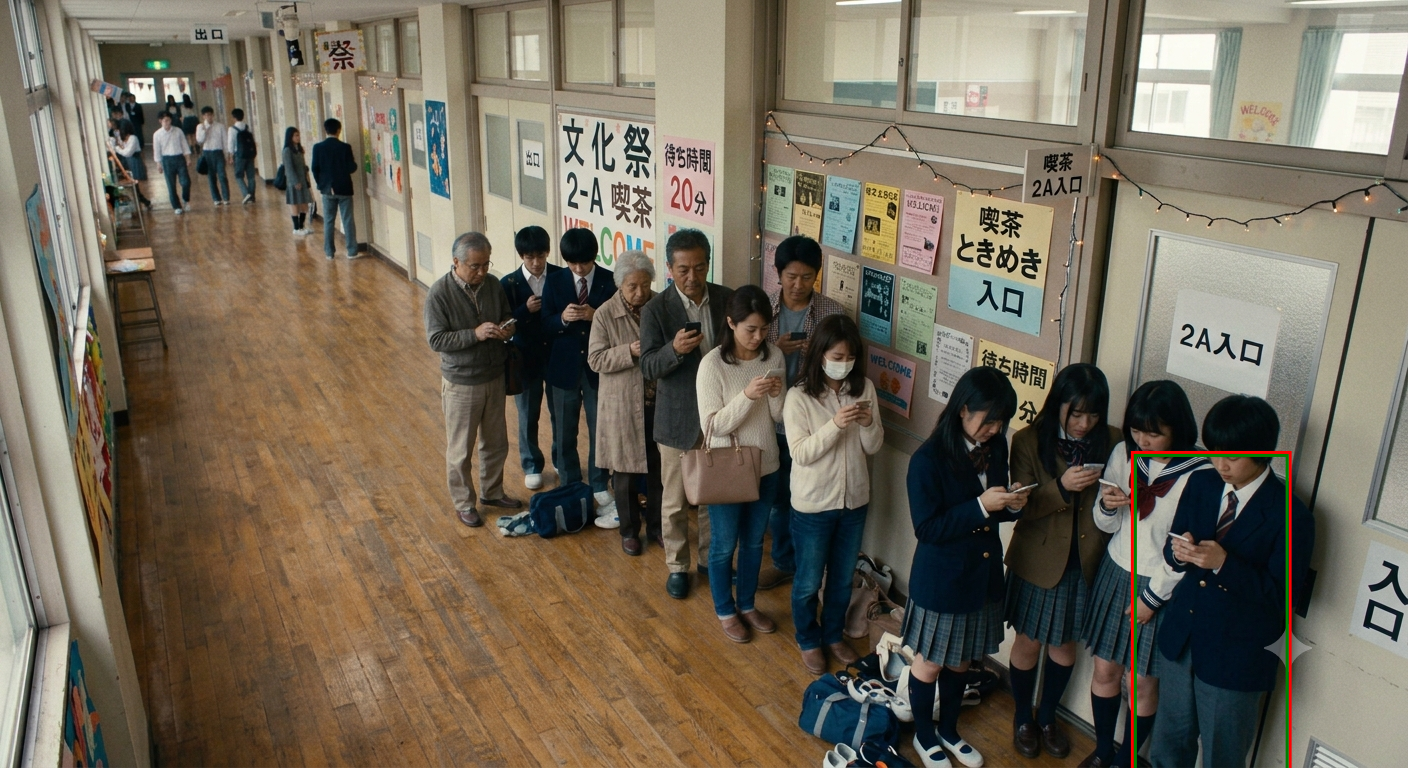
\includegraphics[width=0.25\textwidth]{experiment/results/approach_04_pose_detection/strangers/detection_outputs/annotated_images/t_001s.png}}}$ &
      \jsonlen{experiment/results/approach_04_pose_detection/strangers/detection_outputs/labels/t_001s.json} &
      % 符号と数値
        \ifnum\numexpr \jsonlen{experiment/results/approach_04_pose_detection/strangers/detection_outputs/labels/t_001s.json} - \gtstrangers\relax>0 +\fi\the\numexpr
        \jsonlen{experiment/results/approach_04_pose_detection/strangers/detection_outputs/labels/t_001s.json} - \gtstrangers\relax \\
    
    \hline
    
    $\vcenter{\hbox{視覚的クラッター}}$ &
      $\vcenter{\hbox{\includegraphics[width=0.25\textwidth]{experiment/results/approach_03_face_detection/various_clothes/detection_outputs/annotated_images/t_001s.png}}}$ &
      $\vcenter{\hbox{\includegraphics[width=0.25\textwidth]{experiment/results/approach_04_pose_detection/various_clothes/detection_outputs/annotated_images/t_001s.png}}}$ &
      \jsonlen{experiment/results/approach_04_pose_detection/various_clothes/detection_outputs/labels/t_001s.json} &
      % 符号と数値
        \ifnum\numexpr \jsonlen{experiment/results/approach_04_pose_detection/various_clothes/detection_outputs/labels/t_001s.json} - \gtvariousclothes\relax>0 +\fi\the\numexpr
        \jsonlen{experiment/results/approach_04_pose_detection/various_clothes/detection_outputs/labels/t_001s.json} - \gtvariousclothes\relax \\
    
    \hline

  \end{tabular}
  }
\end{table}

動画を入力データとして検証を行った際の実験結果を表\ref{tab:approach04_video_results}に示す。最も理想的な入力フレームおよびオクルージョン発生時のフレームを掲載している。

\begin{table}[H]
  \centering
  \small
  \caption{アプローチ04：実験結果の比較（動画）}
  \label{tab:approach04_video_results}
  \adjustbox{max width=\textwidth}{%
  \begin{tabular}{|c|c|c|c|c|}

    \hline

      & \begin{tabular}{c} 前アプローチの \\ 検出結果 \end{tabular}
      & 検出結果
      & \begin{tabular}{c} 検出された \\ グループ数 \end{tabular}
      & 実際のグループ数との差 \\
    
    \hline

    $\vcenter{\hbox{理想的な状態}}$ &
      $\vcenter{\hbox{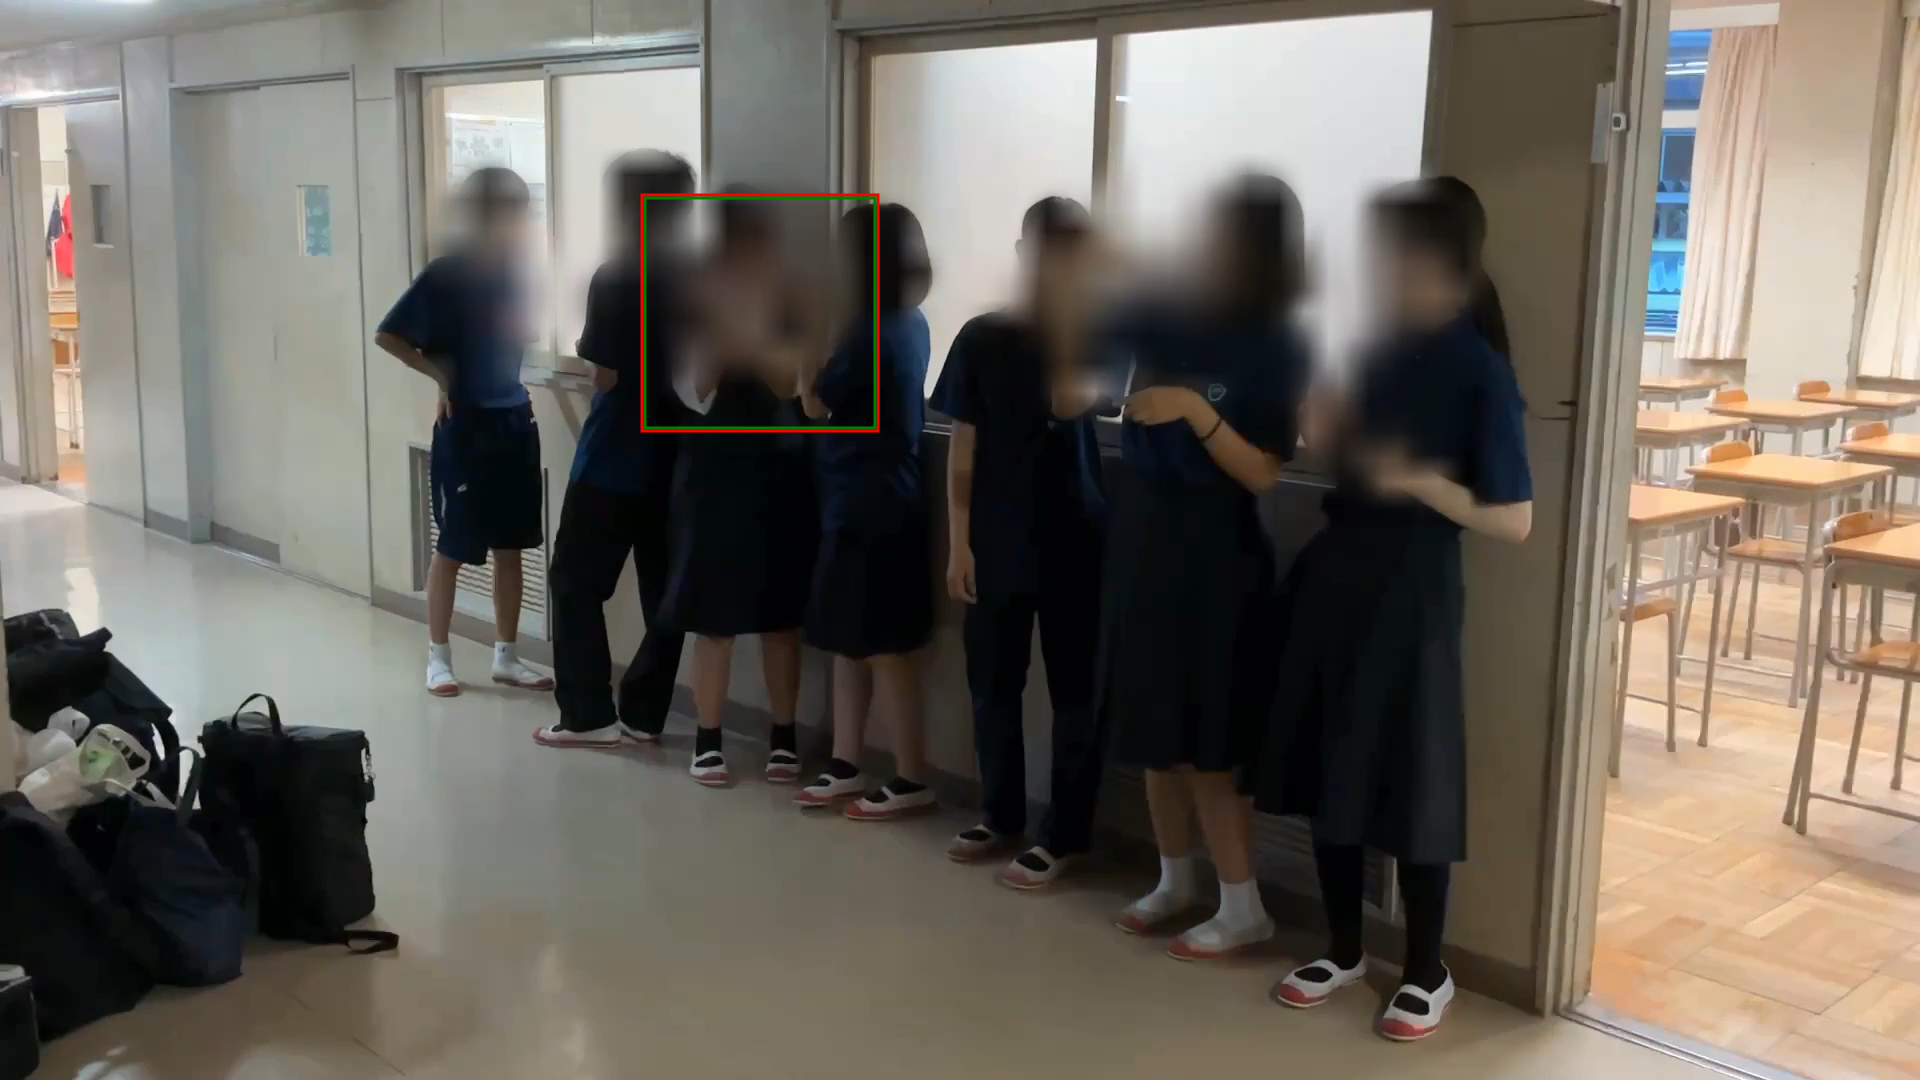
\includegraphics[width=0.25\textwidth]{experiment/results/approach_03_face_detection/queue_video/detection_outputs/annotated_images/t_012s.png}}}$ &
      $\vcenter{\hbox{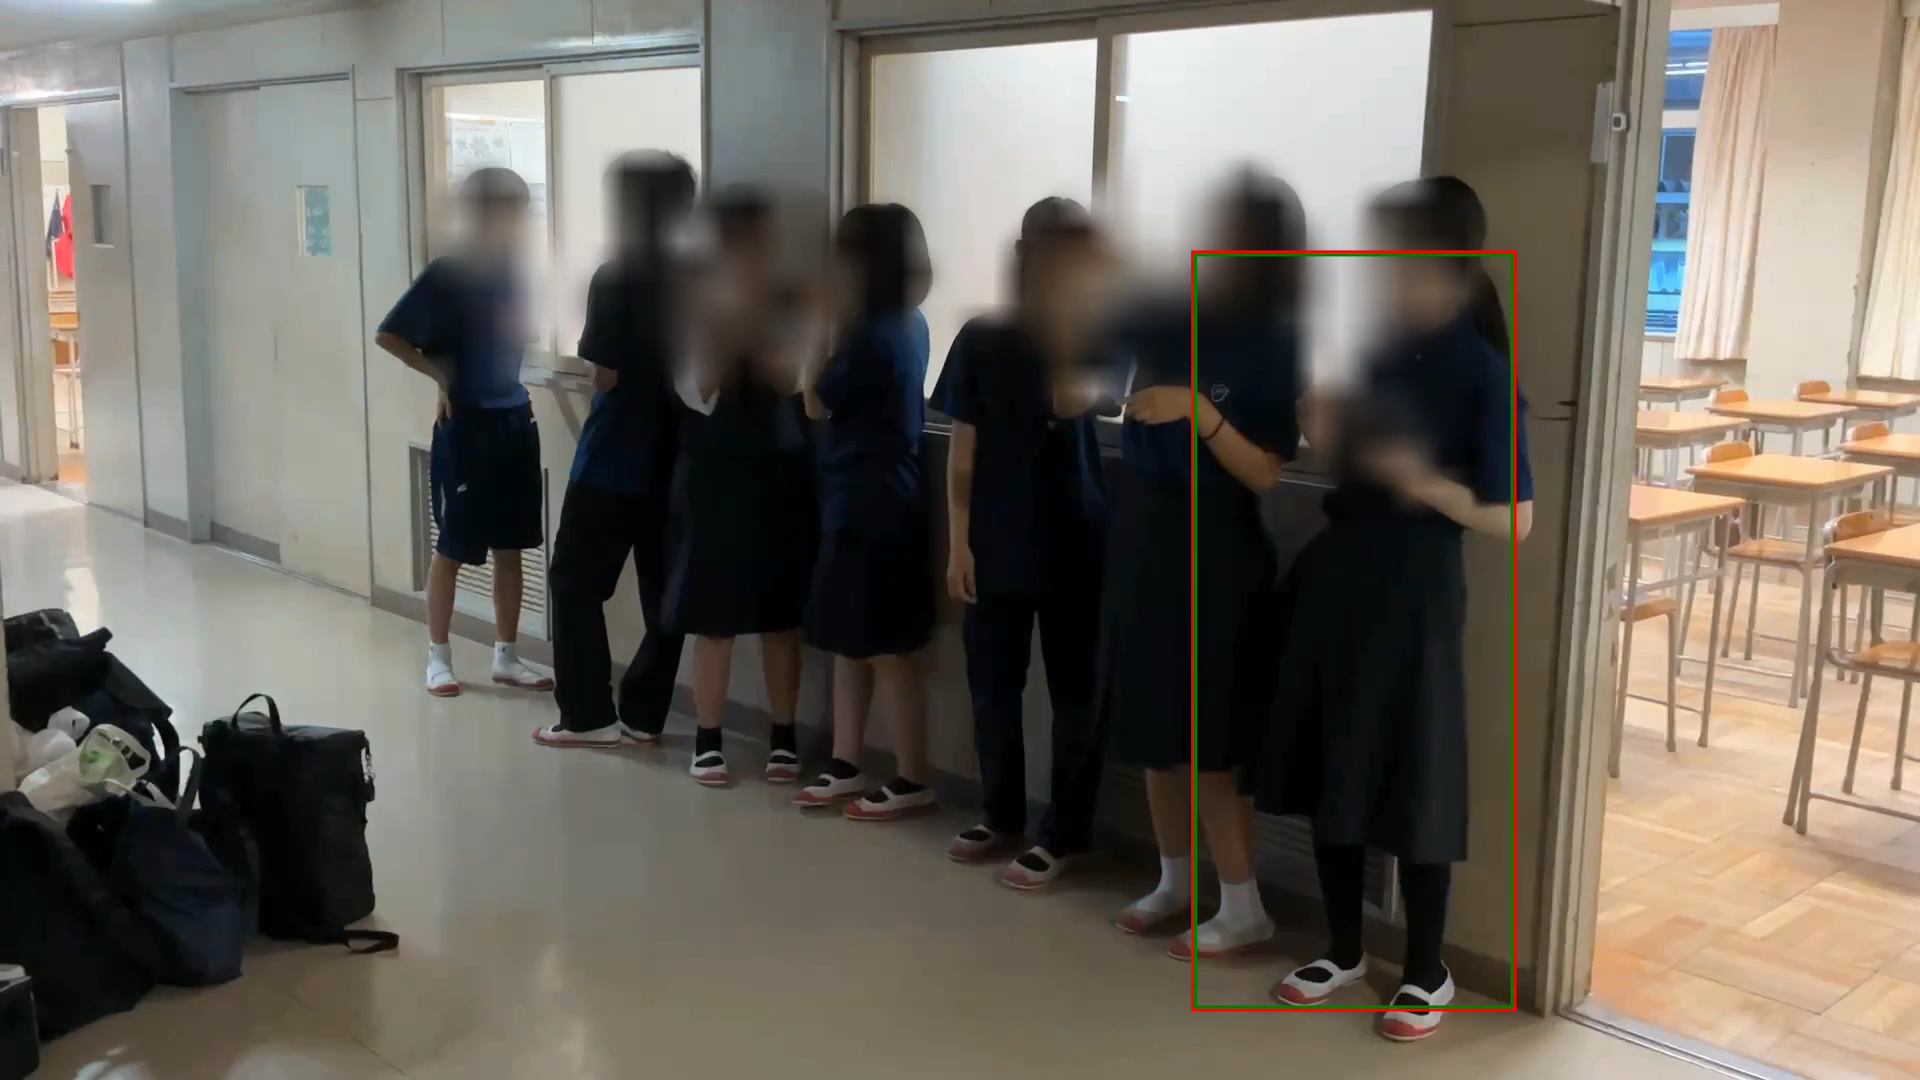
\includegraphics[width=0.25\textwidth]{experiment/results/approach_04_pose_detection/queue_video/detection_outputs/annotated_images/t_012s.png}}}$ &
      \jsonlen{experiment/results/approach_04_pose_detection/queue_video/detection_outputs/labels/t_012s.json} &
      % 符号と数値
        \ifnum\numexpr\jsonlen{experiment/results/approach_04_pose_detection/queue_video/detection_outputs/labels/t_012s.json} - \gtvideoideal\relax>0 +\fi\the\numexpr
        \jsonlen{experiment/results/approach_04_pose_detection/queue_video/detection_outputs/labels/t_012s.json} - \gtvideoideal\relax \\
    
    \hline
    
    $\vcenter{\hbox{オクルージョン発生時}}$ &
      $\vcenter{\hbox{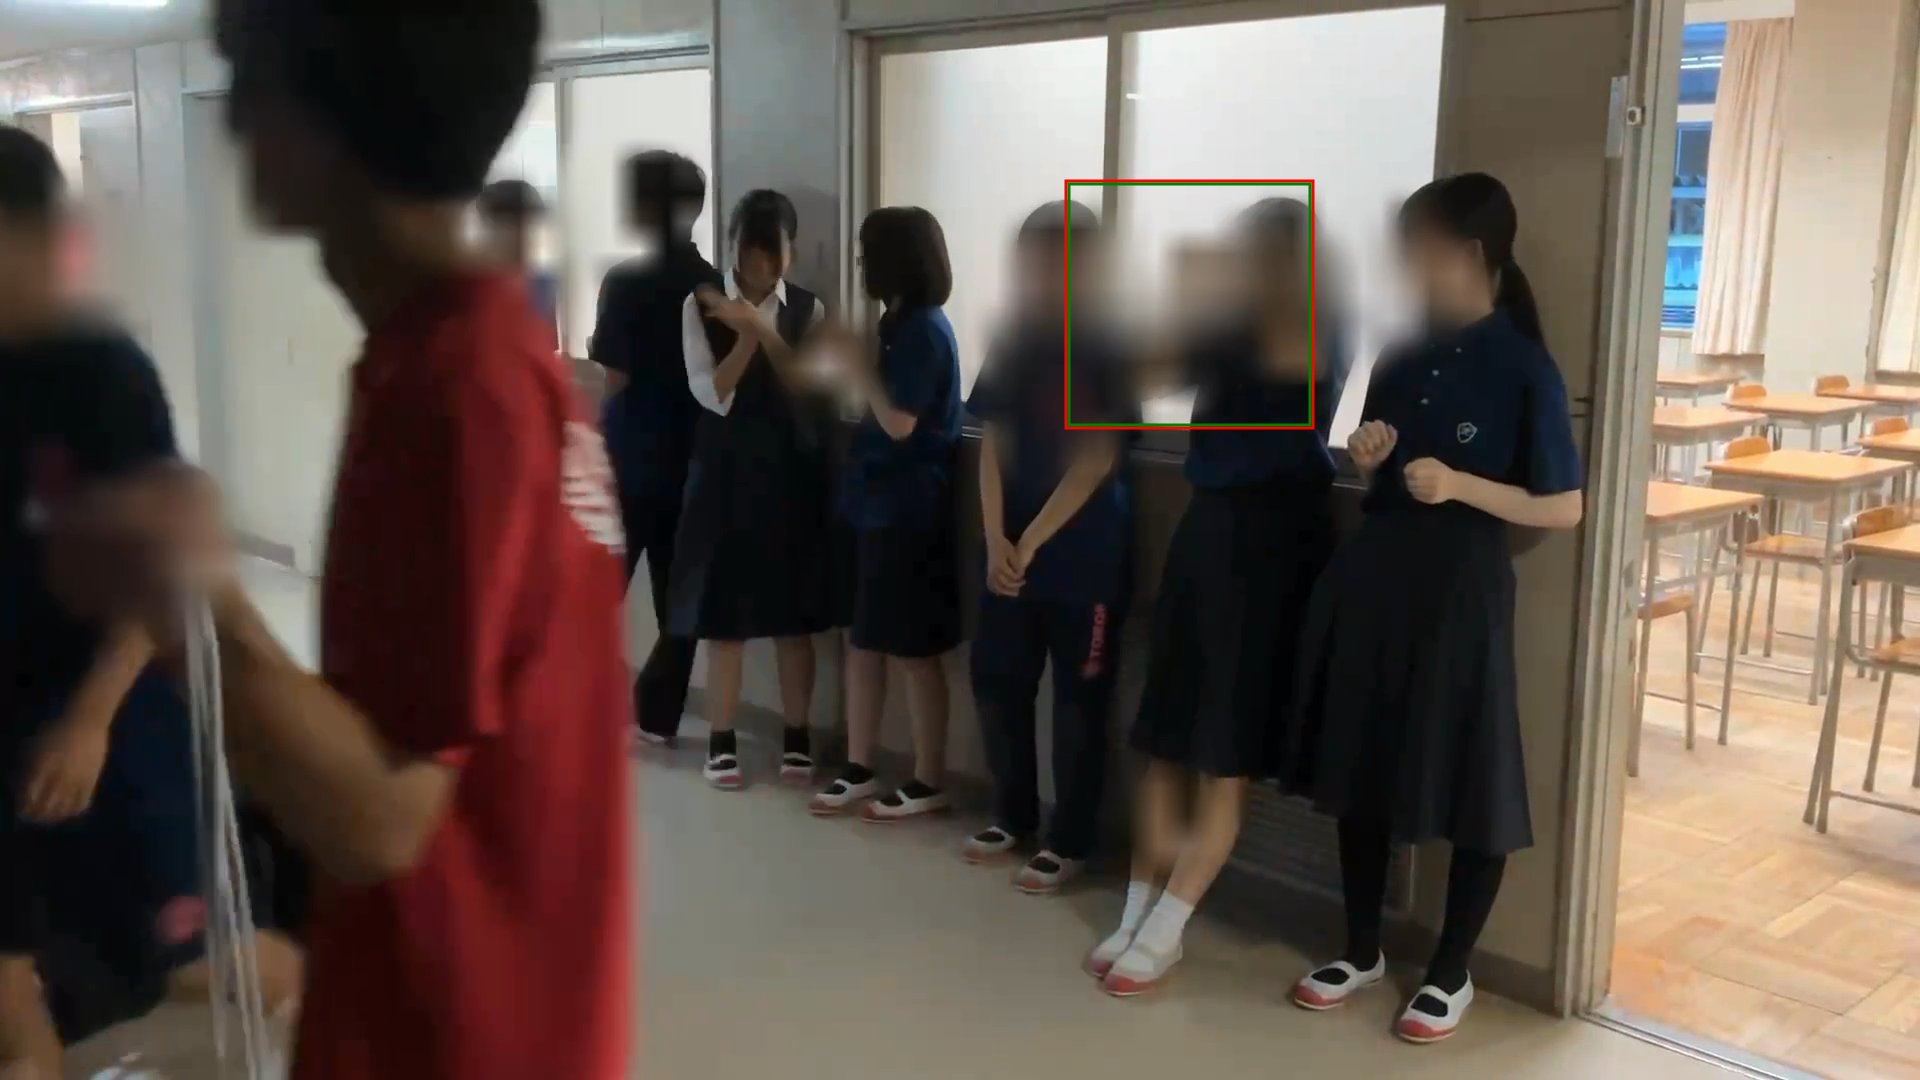
\includegraphics[width=0.25\textwidth]{experiment/results/approach_03_face_detection/queue_video/detection_outputs/annotated_images/t_017s.png}}}$ &
      $\vcenter{\hbox{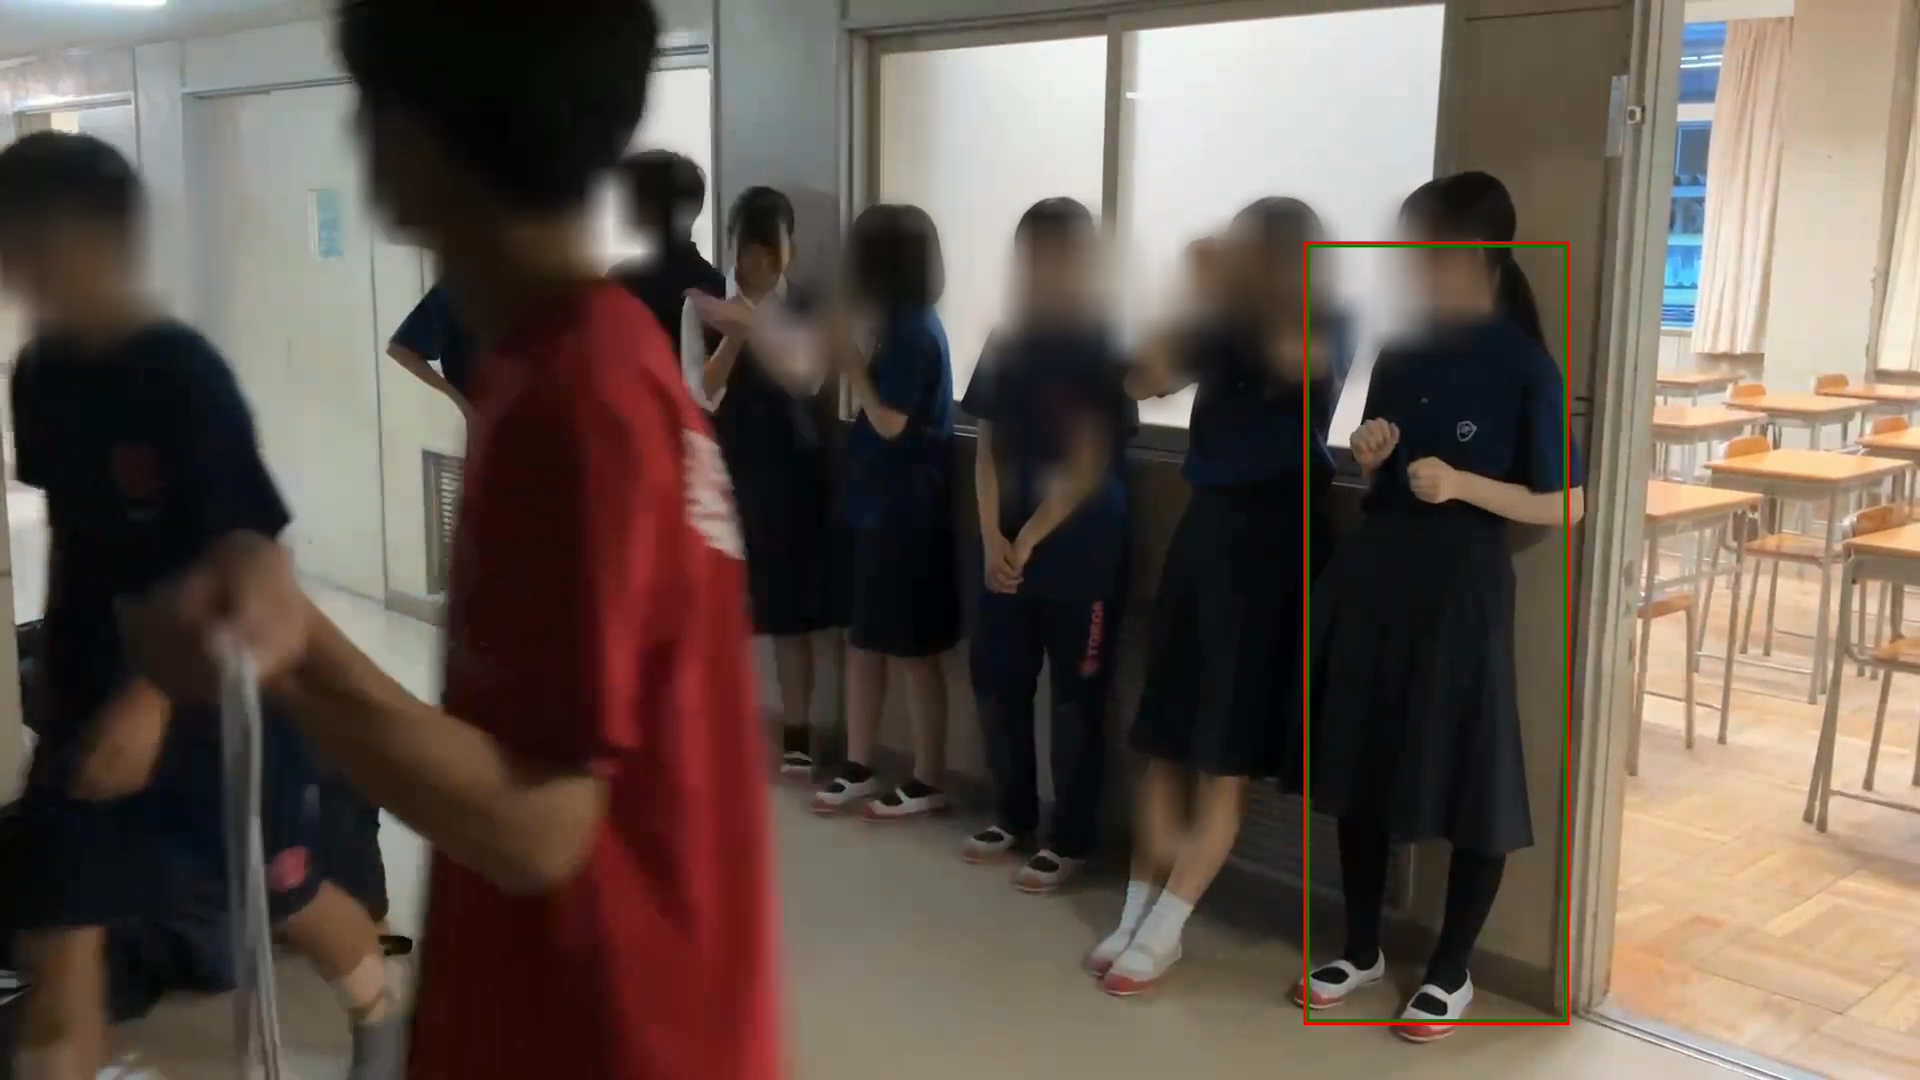
\includegraphics[width=0.25\textwidth]{experiment/results/approach_04_pose_detection/queue_video/detection_outputs/annotated_images/t_017s.png}}}$ &
      \jsonlen{experiment/results/approach_04_pose_detection/queue_video/detection_outputs/labels/t_017s.json} &
      % 符号と数値
        \ifnum\numexpr\jsonlen{experiment/results/approach_04_pose_detection/queue_video/detection_outputs/labels/t_017s.json} - \gtvideoocclusion\relax>0 +\fi\the\numexpr
        \jsonlen{experiment/results/approach_04_pose_detection/queue_video/detection_outputs/labels/t_017s.json} - \gtvideoocclusion\relax \\
    
    \hline
    
  \end{tabular}%
  }
\end{table}

\subsubsection{アプローチ03との比較}
後ろ姿や極度な横向きの姿勢をとる人物に対する検出漏れが大幅に低減された。また、肩や腰の関節点座標を取得できたことにより、単なる位置（二次元座標）にとどまらない「人物の向き」を表現するための基礎情報を保持することが可能となった。

\subsection{課題}
アプローチ04の明瞭となった課題は以下の通りである。

\begin{enumerate}
    \item \textbf{画像全体に対する直接的なポーズ推定の計算コスト}：
    画面全体を直接ポーズ推定モデルに入力する場合、高解像度画像や複数人物が存在する環境下において推論処理の計算負荷が極めて高くなり、フレームレートの維持が困難となった。
    \item \textbf{密集環境でのキーポイント交錯}：
    人物が重なり合う密集部において、異なる人物の関節点同士が誤って関連付けられる現象や、一部のキーポイント検出信頼度が著しく低下する課題が残された。
\end{enumerate}

\clearpage % 視認性のために改ページ挿入
